\documentclass[12pt]{scrartcl}
\usepackage{amsmath}
\usepackage{FiraSans}
\usepackage{siunitx}
\usepackage{hyperref}
\usepackage[capitalise]{cleveref}
\usepackage{graphicx}
\graphicspath{
{./figures/}}
\DeclareGraphicsExtensions{.pdf,.png,.gif}


\newcommand{\myscale}{1}

\begin{document}

\title{Tomography reconstruction of }
\author{Chen Zhang}

\maketitle

% ---- Background -----
\section{Background}\label{sec: bg}

\section{Experiment}\label{sec: exp}

\section{Tomography reconstruction}\label{sec: tomo}

\subsection{Data preprocessing}\label{sec: preprocessing}

\subsubsection{Background normalization}\label{sec: bg norm}

% --- background images --- %
\renewcommand{\myscale}{0.8}
\begin{figure}
\centering
\begin{tabular}{cc}
	 White field (before)
&  White field difference
\\
  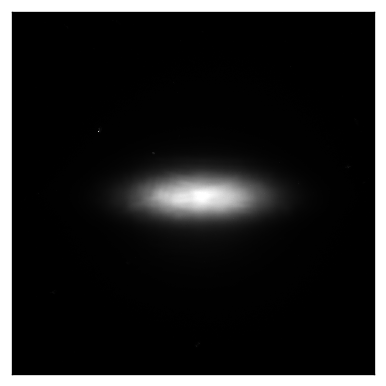
\includegraphics[scale=\myscale]{whiteField_pre} 
& 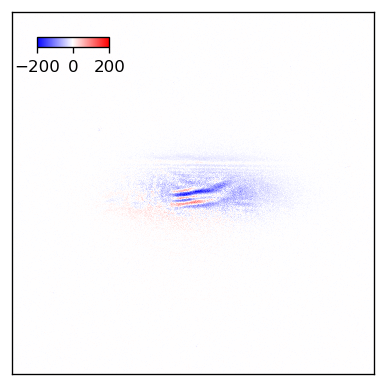
\includegraphics[scale=\myscale]{whiteField_diff}
\\
	Dark field (after)
& White field (after)
\\
	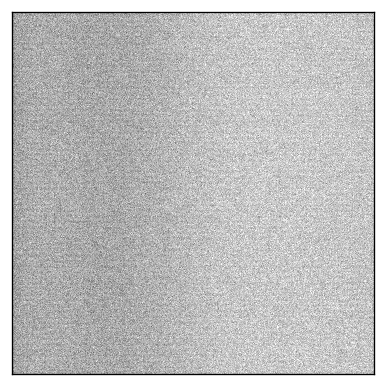
\includegraphics[scale=\myscale]{darkField_pst}
& 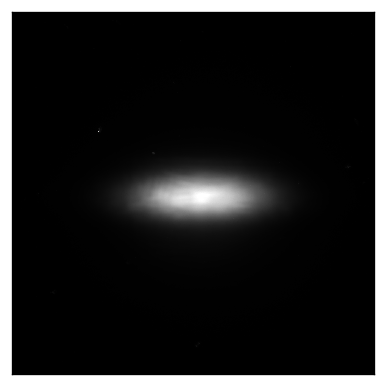
\includegraphics[scale=\myscale]{whiteField_pst}
\end{tabular}
\caption{
The median of background (white and dark) images collected before and after the tomography scan.
The dynamic range of the white field images are $[0,4000]$ (counts) while the dynamic range of the dark field image is $[0,10]$ (counts).
}
\end{figure}


\subsubsection{Data correction}\label{sec: data correction}

% --- corrupted frame detection
\renewcommand{\myscale}{1}
\begin{figure}
\centering
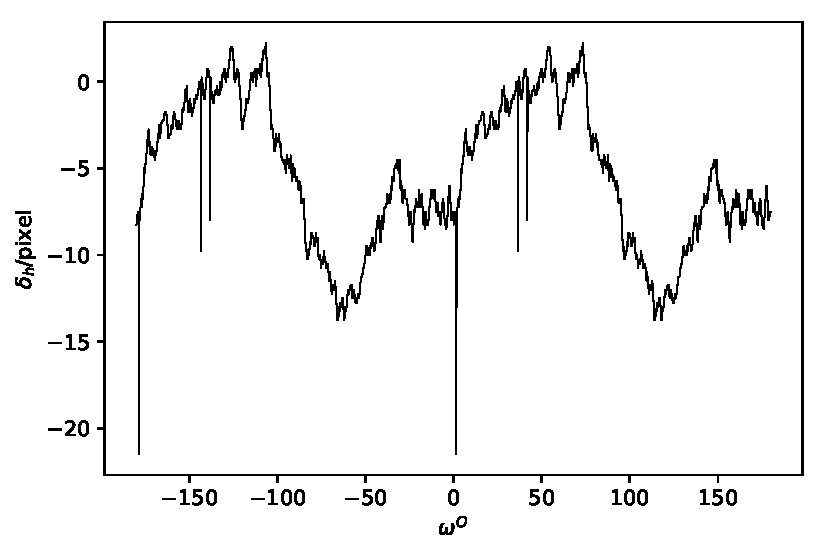
\includegraphics[scale=\myscale]{corruptedFrameDetection}
\caption{
The corrupted frames can be detected by checking the outliers in the profile of \ang{180} pair-wise rotation axis where $\delta_h$ denotes the amount of horizontal offset between rotation axis and the image center column.
}\label{fig: corrupted frame detection}
\end{figure} 

% --- detected corrupted frames
\renewcommand{\myscale}{0.5}
\begin{figure}
\centering
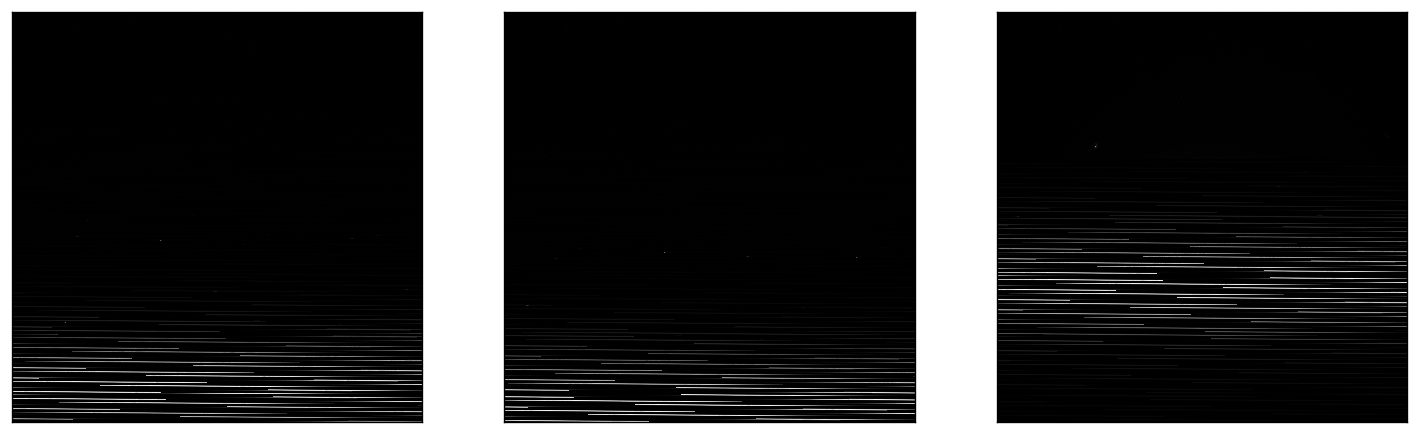
\includegraphics[scale=\myscale]{corruptedFrames}
\caption{
Three corrupted frames were detected out of the total 3600 frames.
Due to the horizontal detector jittering, these corrupted frames and the associated \ang{180} pairs were excluded from the tomography reconstruction as it is not possible to adjust a \ang{180} pair horizontally with one corrupted frame.
}\label{fig: corrupted frames}
\end{figure}

\subsubsection{Data reduction}\label{sec: data reduction}

\subsubsection{Background normalization}\label{sec: bg norm}

\subsubsection{Impulse noise reduction}\label{sec: noise reduction}

% --- noise reduction
\renewcommand{\myscale}{1}
\begin{figure}
\centering
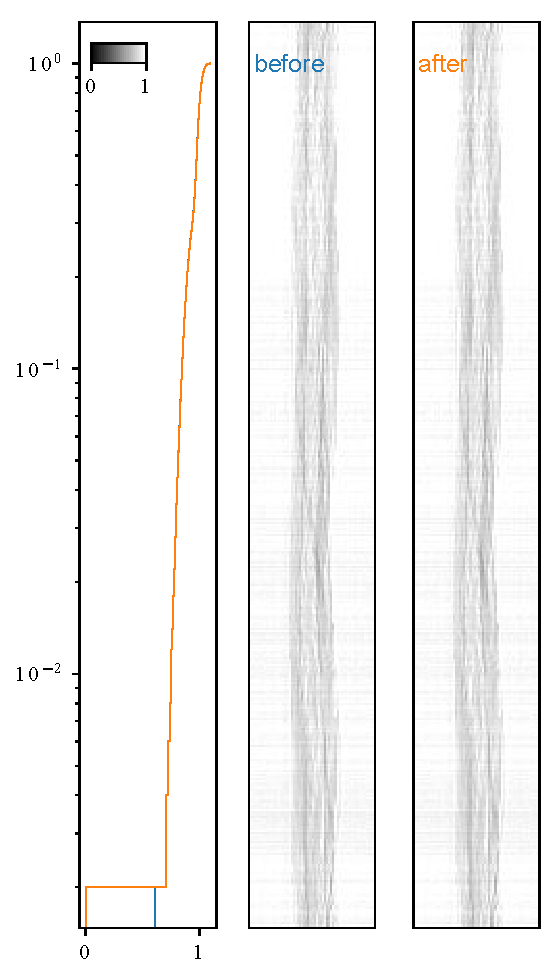
\includegraphics[scale=\myscale]{sinogramDenoise_retouched}
\caption{
Remove impulse noise from sinogram using selective median filter.
}\label{fig: noise reduction}
\end{figure}

\subsubsection{Bcakground level normalization}\label{sec: bg lv norm}

% --- bg lvl norm
\renewcommand{\myscale}{0.5}
\begin{figure}
\centering
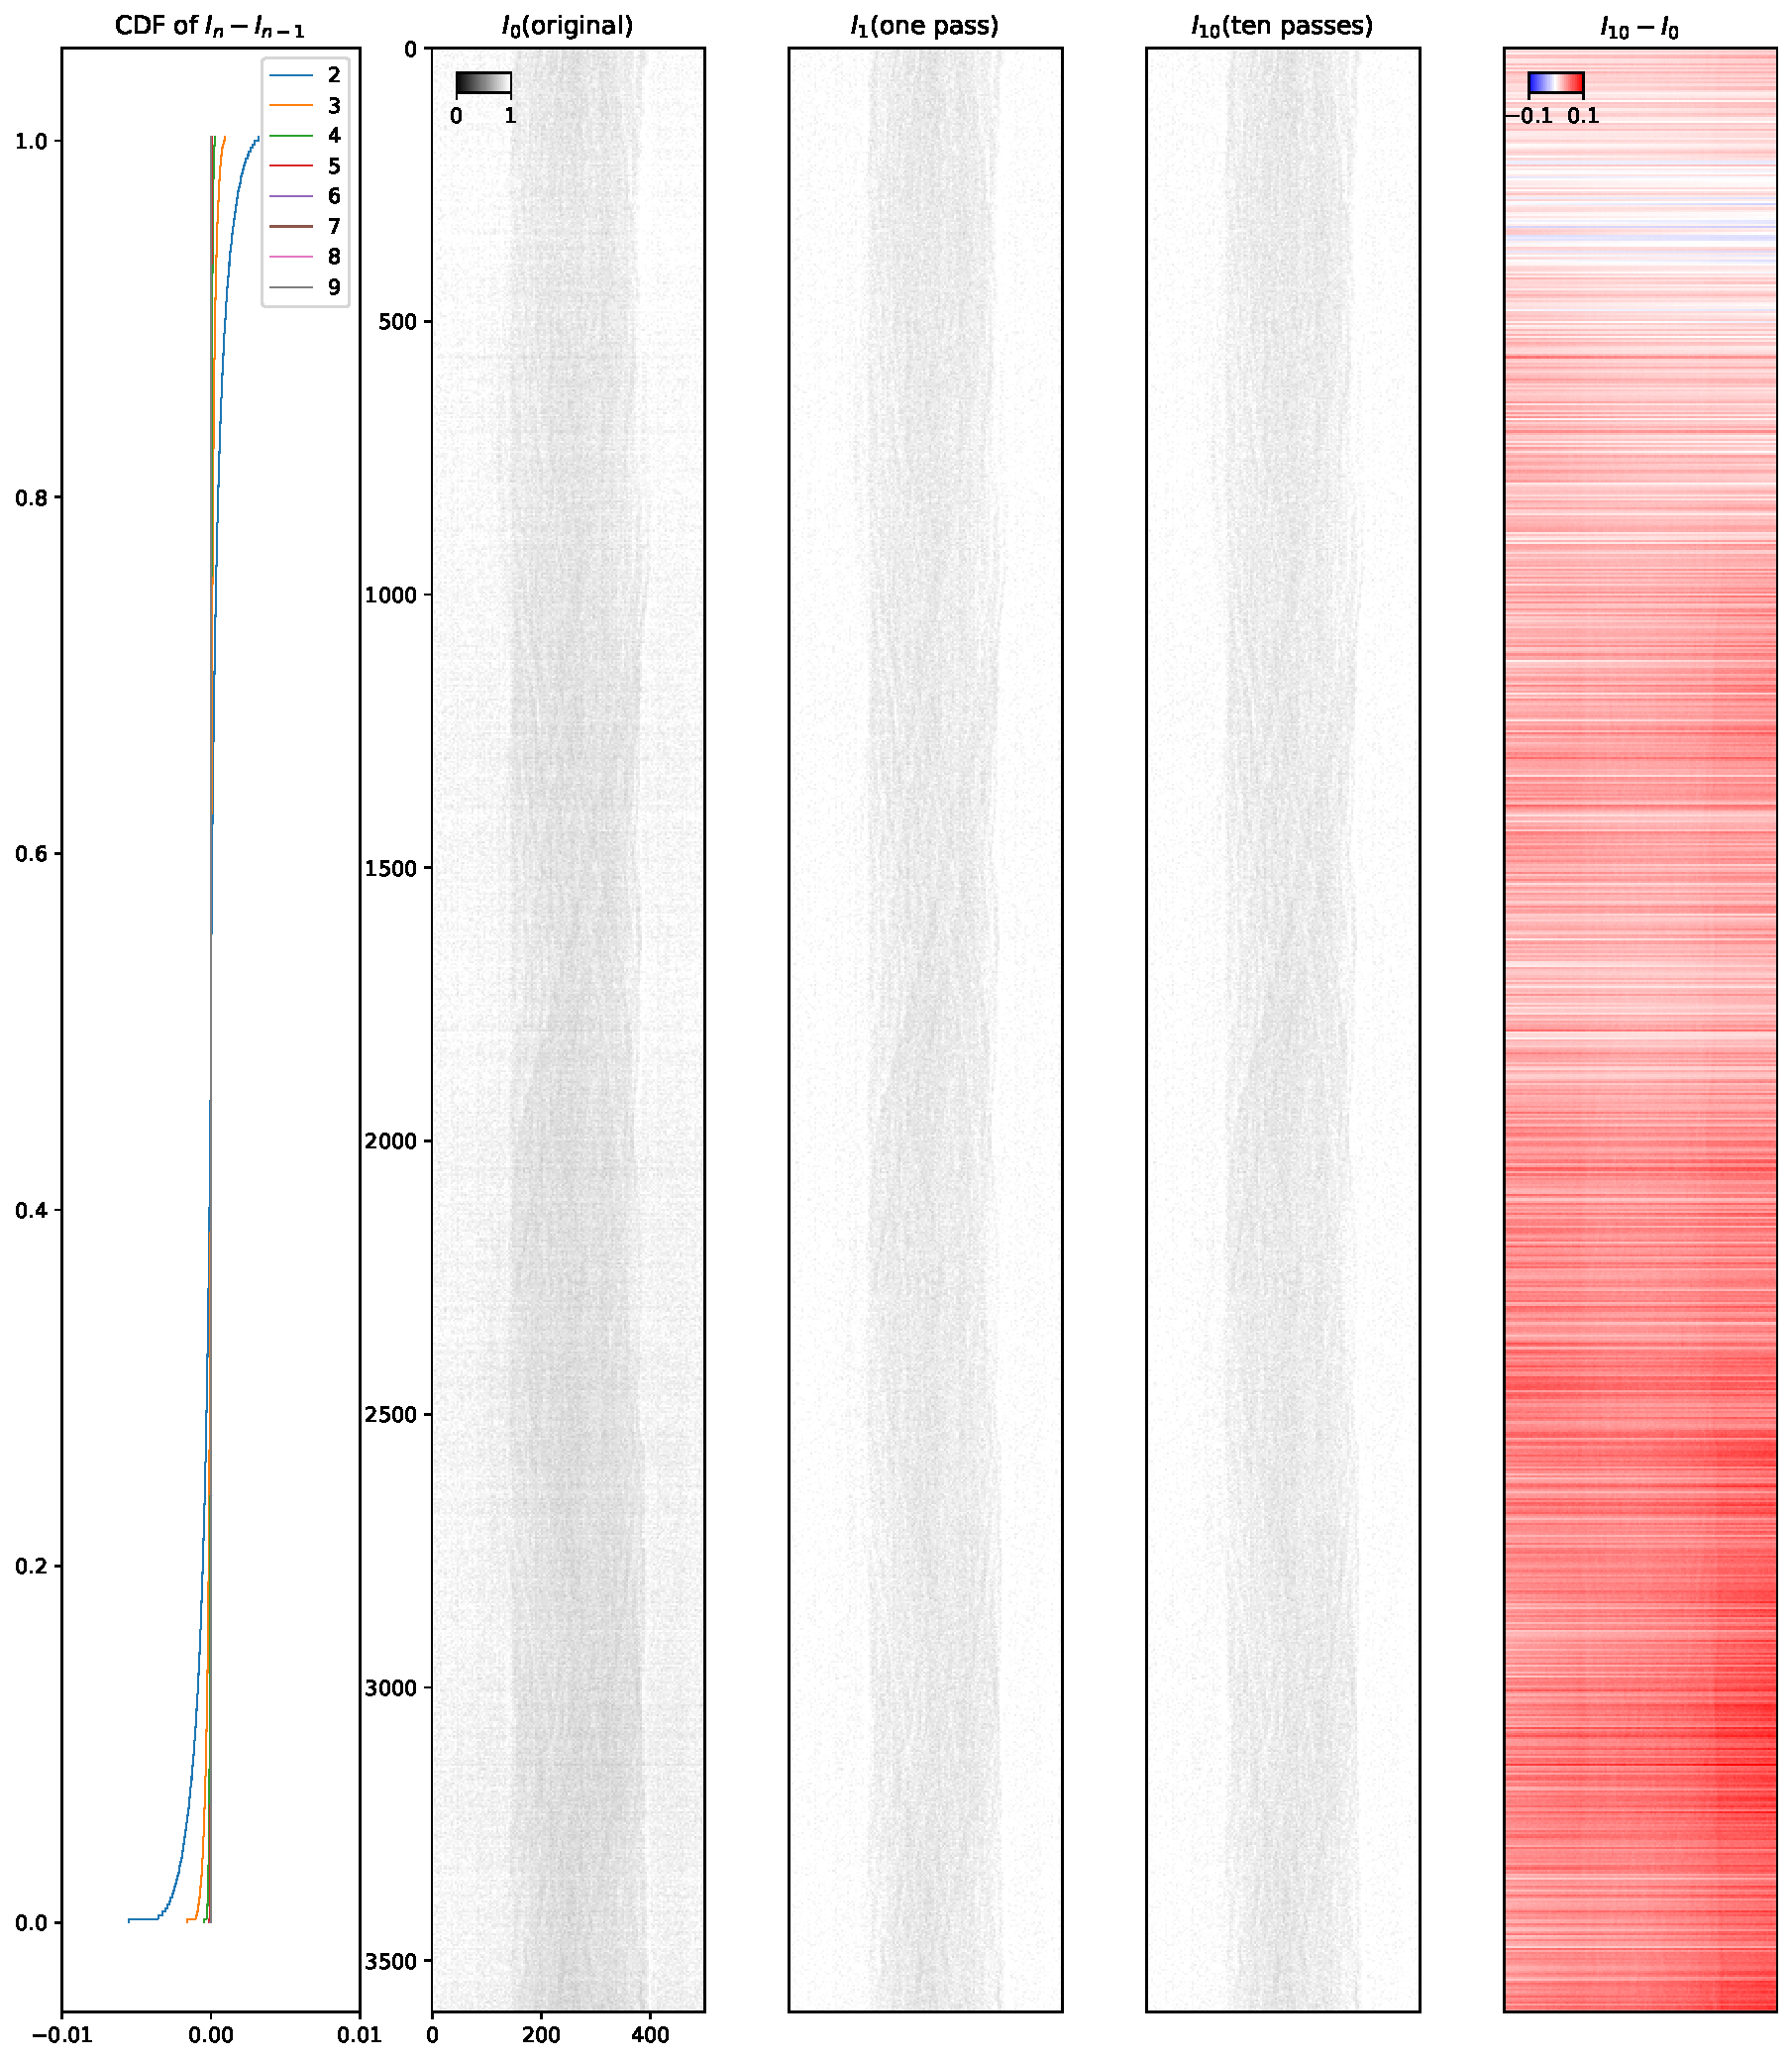
\includegraphics[scale=\myscale]{sinogramNormalization_top}
\caption{
Top region
}\label{fig: sino norm top}
\end{figure}

\begin{figure}
\centering
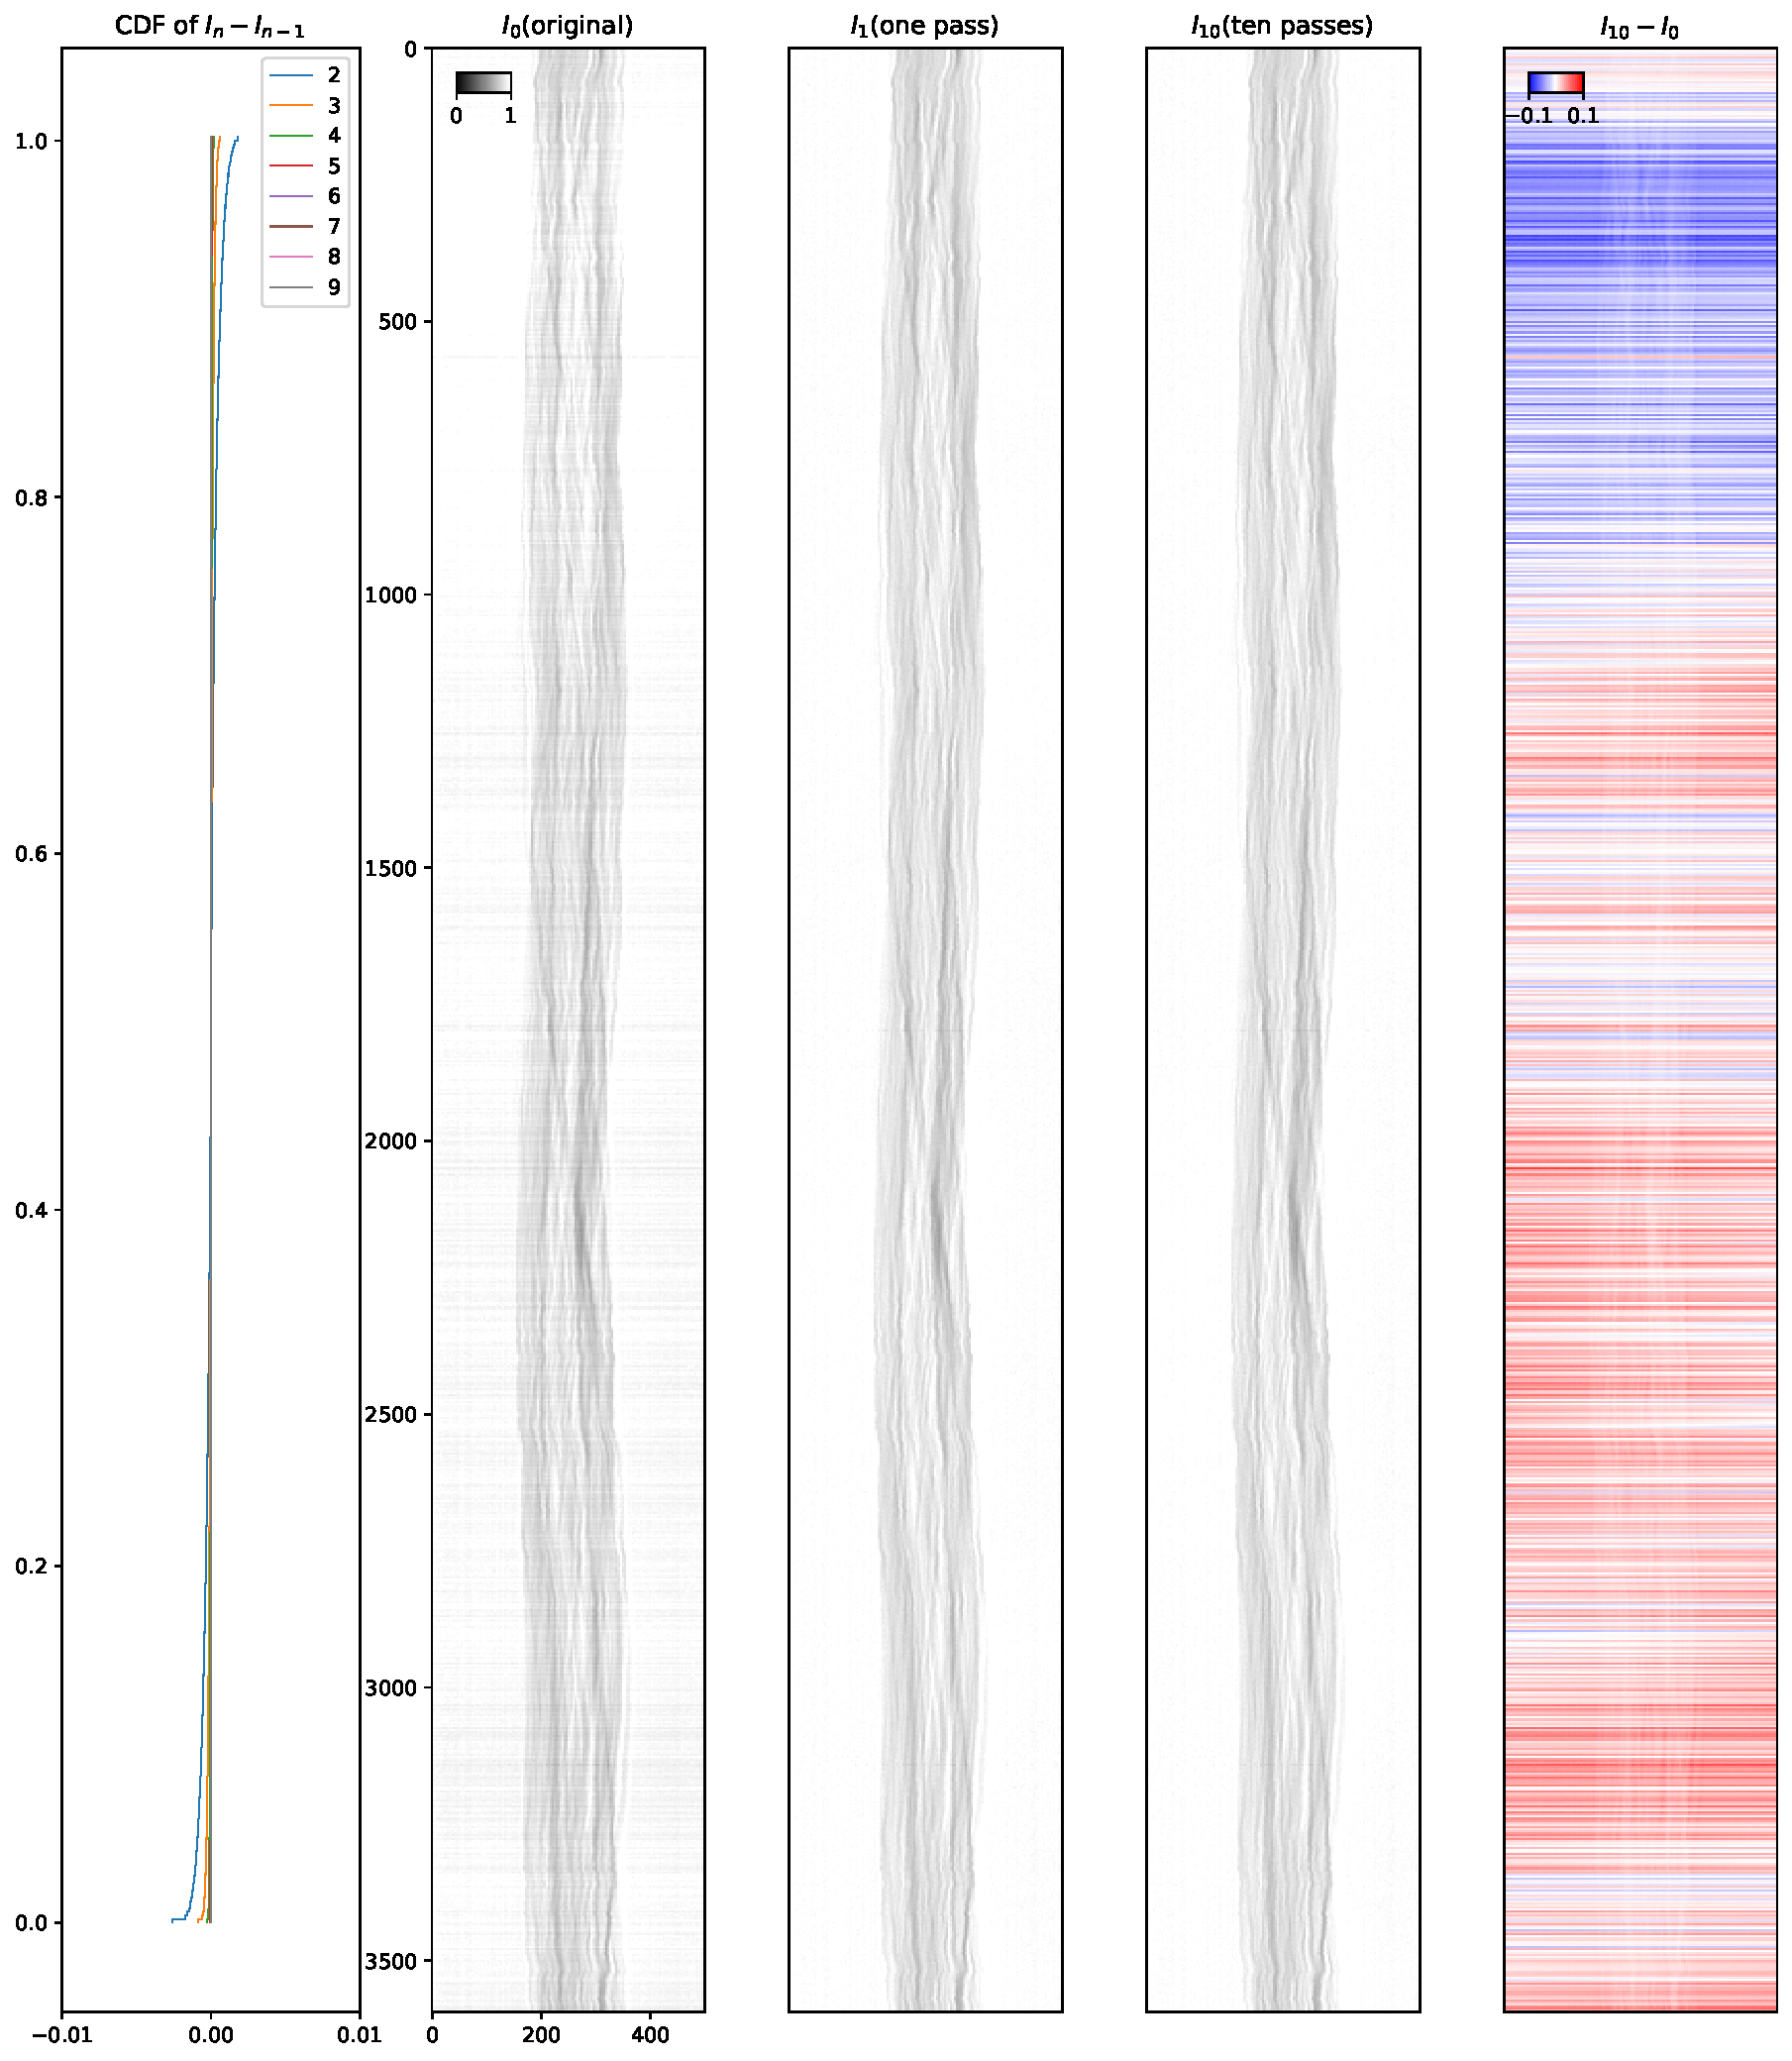
\includegraphics[scale=\myscale]{sinogramNormalization_middle}
\caption{
Middle region
}\label{fig: sino norm mid}
\end{figure}

\begin{figure}
\centering
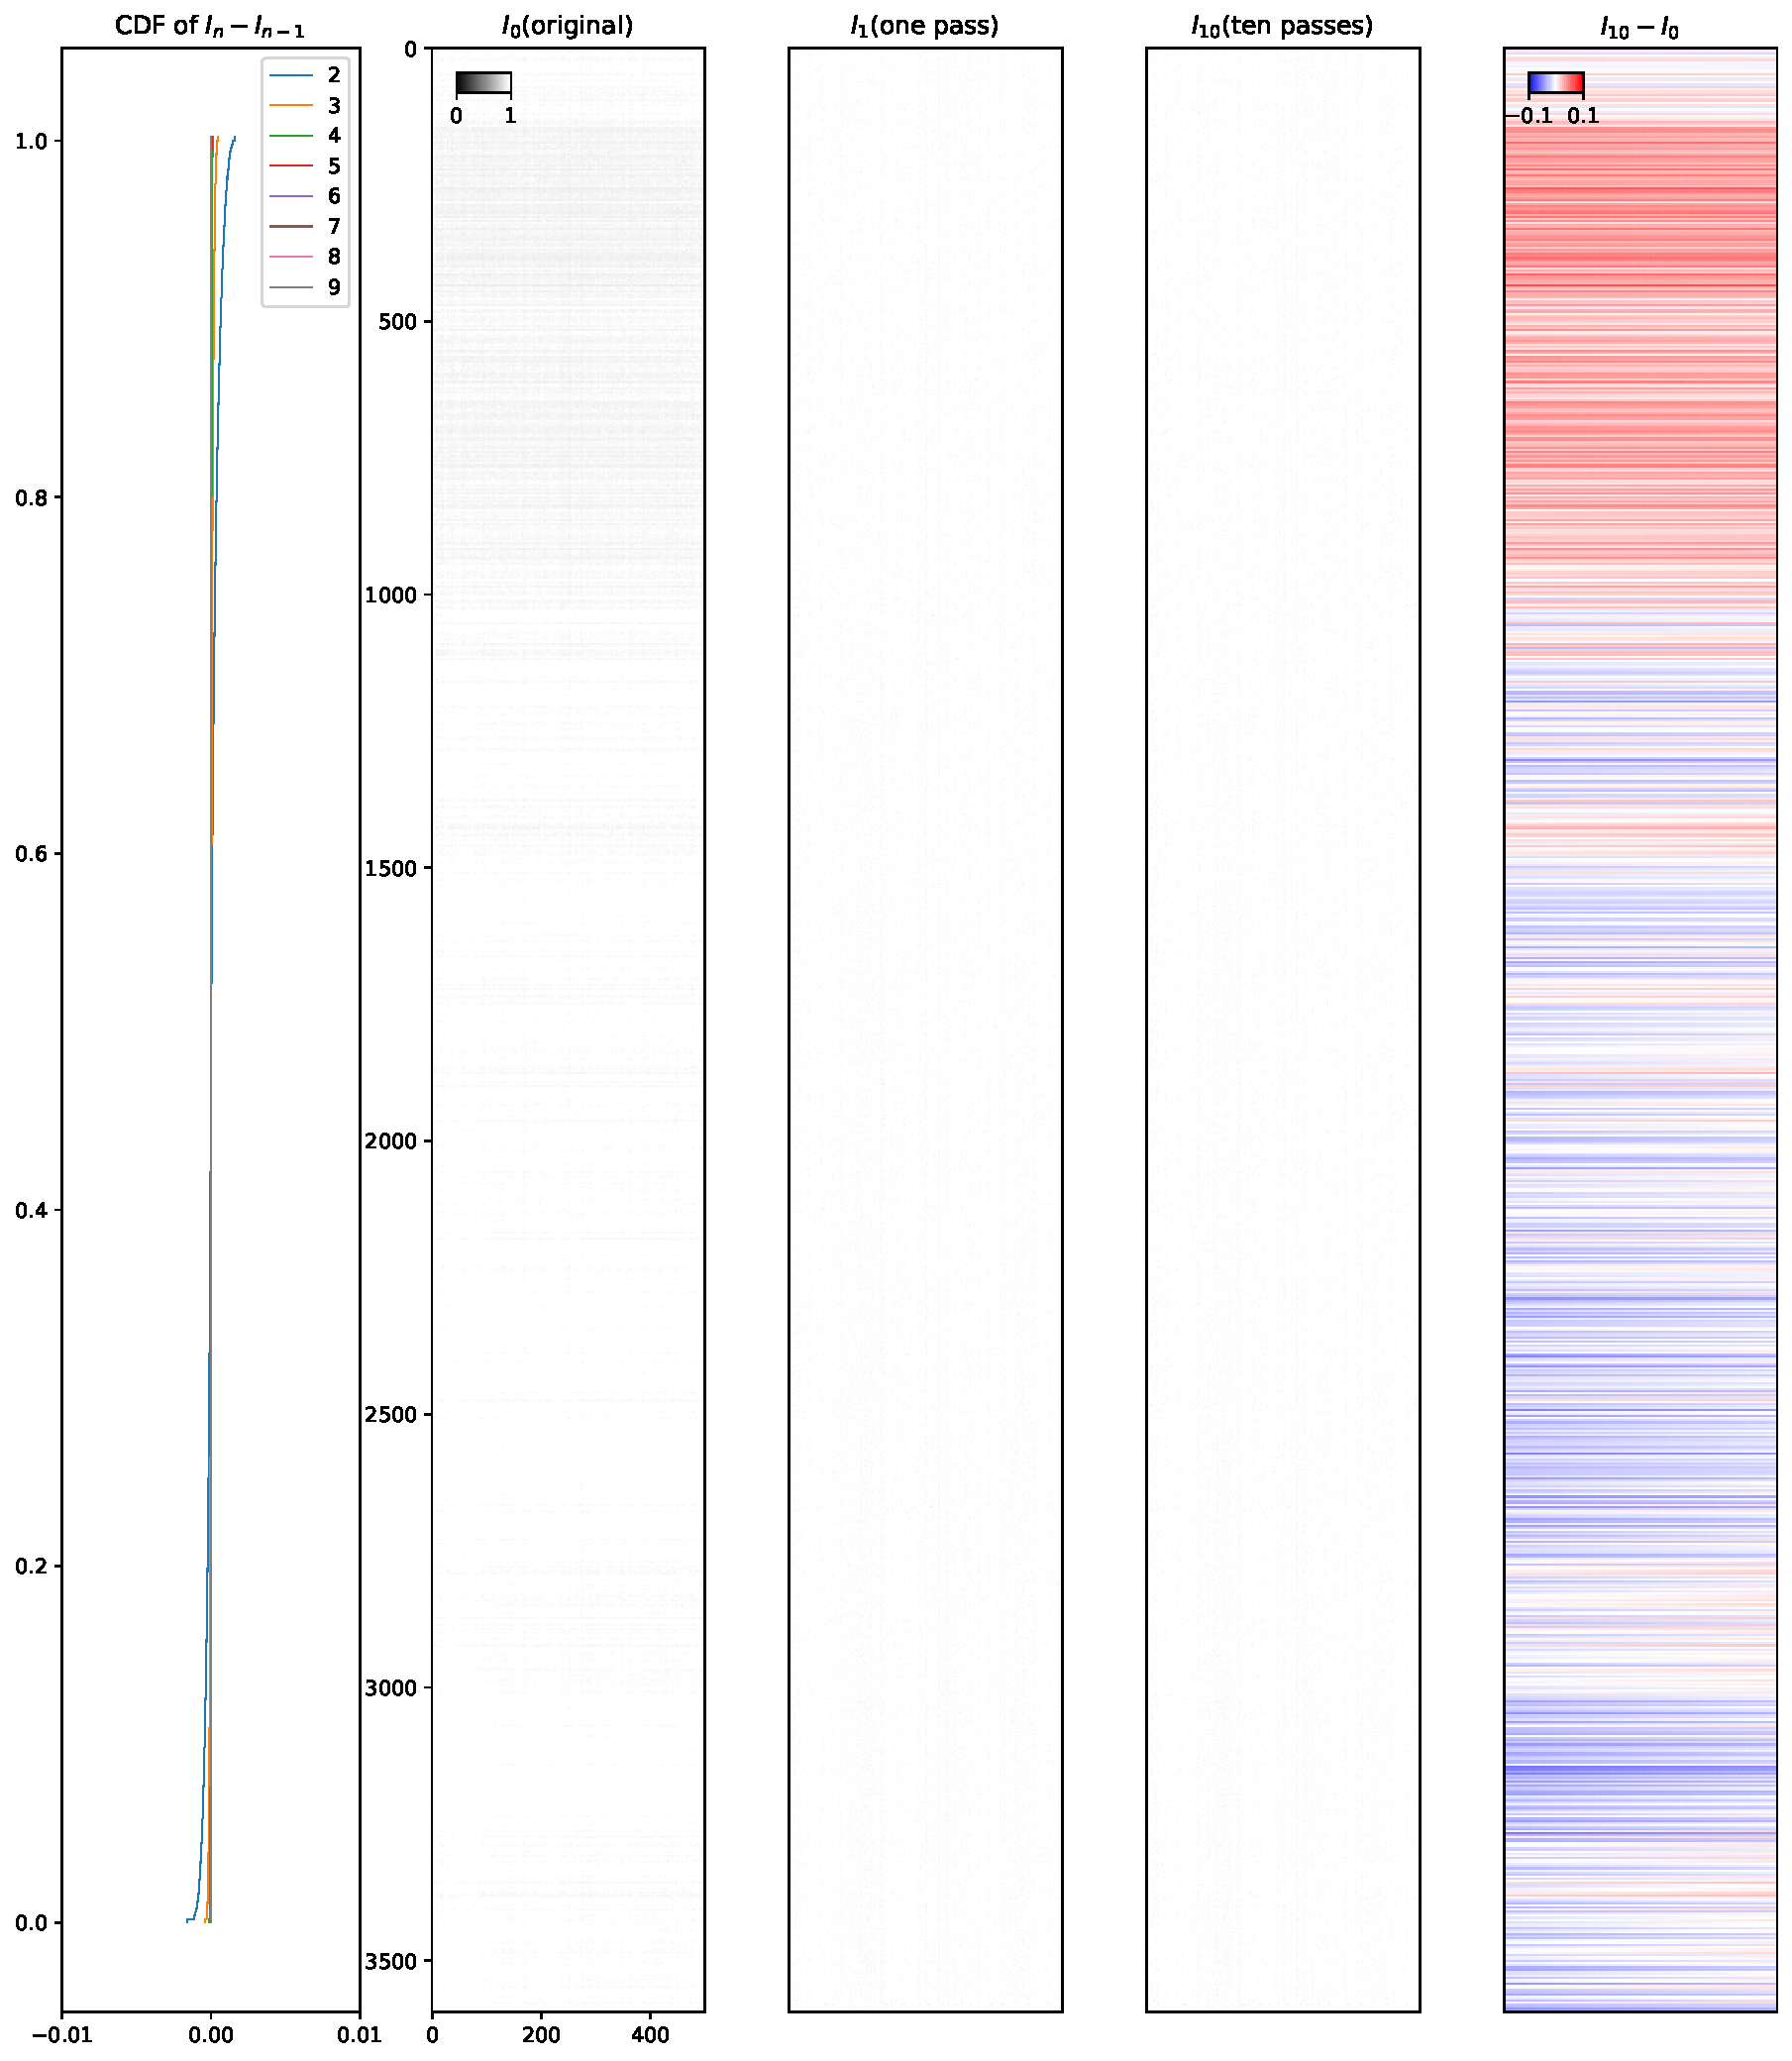
\includegraphics[scale=\myscale]{sinogramNormalization_bottom}
\caption{
Bottom region
}\label{fig: sino norm bot}
\end{figure}

% --- intensity distribution along stack

\section{Porosity characterization}\label{sec: porosity characterization}

% --- void detection demo
\renewcommand{\myscale}{1.0}
\begin{figure}
\centering
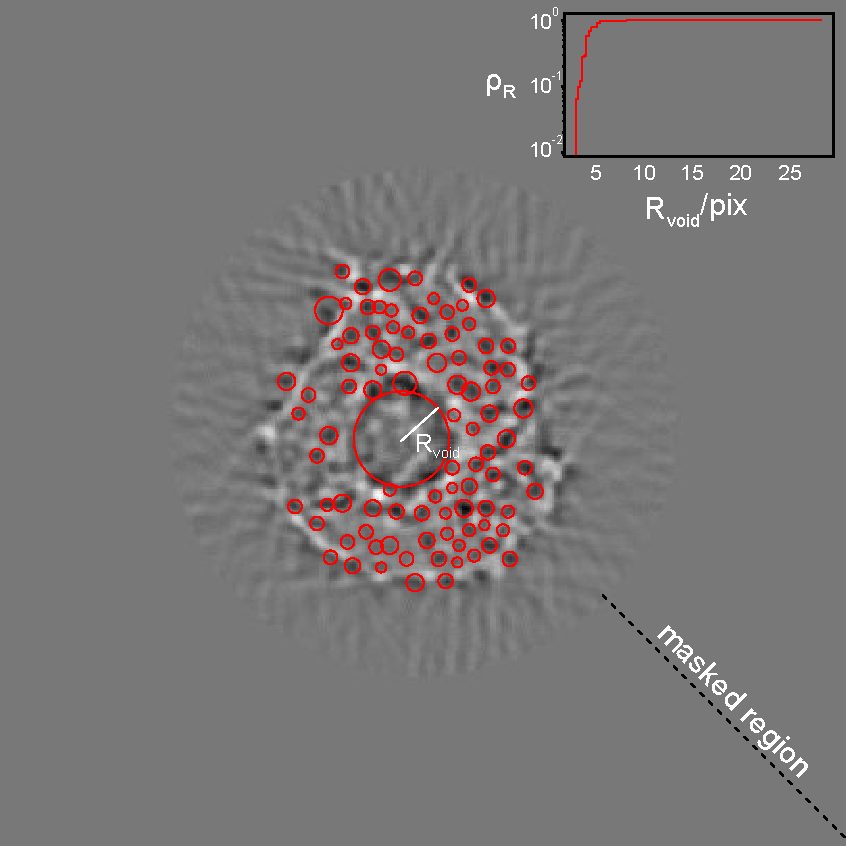
\includegraphics[scale=\myscale]{voidDetectionDemo_mid}
\caption{
void detection demo
}\label{fig: void detection demo}
\end{figure}

% --- porosity profile
\renewcommand{\myscale}{1.0}
\begin{figure}
\centering
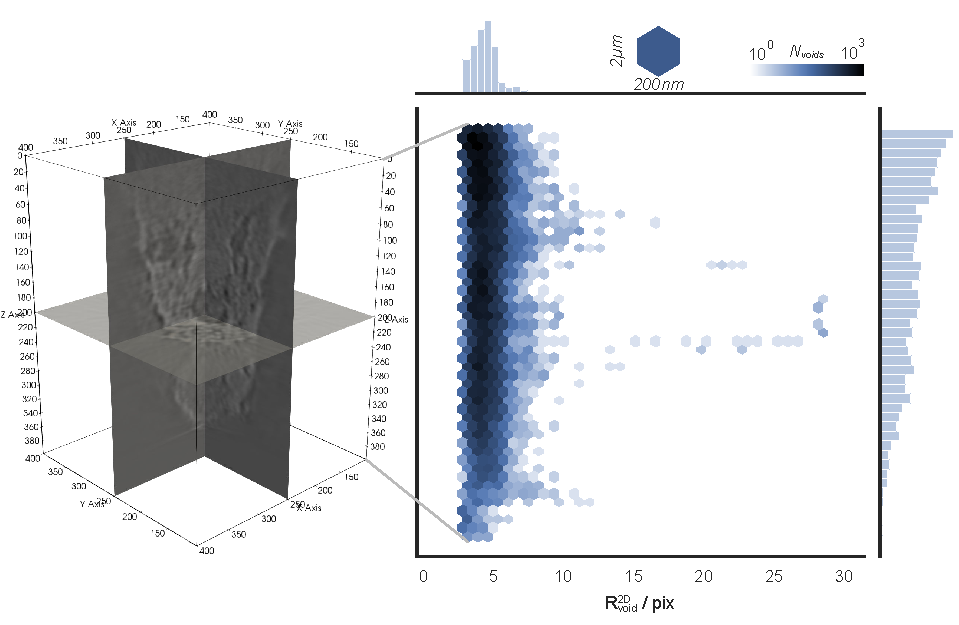
\includegraphics[scale=\myscale]{void_profile}
\caption{
void profile
}\label{fig: void profile}
\end{figure}

\section{Summary}\label{sec: summary}

\end{document}
